%%%%%%%%%%%%%%%%%%%%%%%%%%%%%%%%%%%%%%%%%%%%%%%%%%%%%%%%%%%%%%%%%%%%%%%%%%%%%%%%
%
%   Basic configuration
%
%%%%%%%%%%%%%%%%%%%%%%%%%%%%%%%%%%%%%%%%%%%%%%%%%%%%%%%%%%%%%%%%%%%%%%%%%%%%%%%%

% Use 'KOMA-Script Book' as the document class
\documentclass[toc=bibliography,toc=indentunnumbered]{scrbook} 

% All modern documents should start with this (unless you use XeTeX/LuaTeX)
\usepackage[utf8]{inputenc}      % UTF-8 file encoding
\usepackage[T1]{fontenc}         % 8-bit font encoding

% This package is useful for modding standard environments
\usepackage{etoolbox}



%%%%%%%%%%%%%%%%%%%%%%%%%%%%%%%%%%%%%%%%%%%%%%%%%%%%%%%%%%%%%%%%%%%%%%%%%%%%%%%%
%
%   Page design
%
%%%%%%%%%%%%%%%%%%%%%%%%%%%%%%%%%%%%%%%%%%%%%%%%%%%%%%%%%%%%%%%%%%%%%%%%%%%%%%%%

% Font size
\KOMAoptions{fontsize=11pt}

% Line spacing
\linespread{1.05}

% Paper format
\KOMAoptions{paper=B5}

% Duplex layout
\KOMAoptions{twoside}

% Binding correction
\KOMAoptions{BCOR=12mm}

% Page layout
\KOMAoptions{DIV=11}

% Disable headers
\pagestyle{plain}

% Page numbers
\addtokomafont{pagenumber}{\footnotesize\sffamily\bfseries}

% Left-justify equations
\PassOptionsToPackage{fleqn}{amsmath}

% Use spacing instead of indentation to separate paragraphs
%\KOMAoptions{parskip=half+}



%%%%%%%%%%%%%%%%%%%%%%%%%%%%%%%%%%%%%%%%%%%%%%%%%%%%%%%%%%%%%%%%%%%%%%%%%%%%%%%%
%
%   Document fonts
%
%%%%%%%%%%%%%%%%%%%%%%%%%%%%%%%%%%%%%%%%%%%%%%%%%%%%%%%%%%%%%%%%%%%%%%%%%%%%%%%%

% Palatino serif font (main text font)
\usepackage[largesc]{newpxtext}

% Optima sans font (titles, captions, footnotes, and links)
\usepackage{classico}

% Euler mathematical font (math)
\usepackage[utf8]{eulerpx/eulerpx}

% Vera monospaced font (code)
\usepackage[scaled=0.84]{beramono}

% Enable microtypographic tweaks
\usepackage{microtype}

% Ensure that we always combine sans text and math
\let\oldsffamily=\sffamily
\renewcommand{\sffamily}{\oldsffamily\sfmath}



%%%%%%%%%%%%%%%%%%%%%%%%%%%%%%%%%%%%%%%%%%%%%%%%%%%%%%%%%%%%%%%%%%%%%%%%%%%%%%%%
%
%   Table of contents
%
%%%%%%%%%%%%%%%%%%%%%%%%%%%%%%%%%%%%%%%%%%%%%%%%%%%%%%%%%%%%%%%%%%%%%%%%%%%%%%%%
 
% Load a package for styling the table of contents
\usepackage{tocstyle}

% Place page numbers right after the section entries
\usetocstyle{nopagecolumn}

% Do not include subsections in the table of contents
\setcounter{tocdepth}{1}

% Use tabular lining figures for the sections, but oldstyle figures for the pages
\settocstylefeature{entryhook}{\tlfstyle}
\settocstylefeature{pagenumberhook}{\osfstyle}
\settocstylefeature[0]{entryhook}{\tlfstyle\bfseries}
\settocstylefeature[0]{pagenumberhook}{\osfstyle\bfseries}



%%%%%%%%%%%%%%%%%%%%%%%%%%%%%%%%%%%%%%%%%%%%%%%%%%%%%%%%%%%%%%%%%%%%%%%%%%%%%%%%
%
%   Headings
%
%%%%%%%%%%%%%%%%%%%%%%%%%%%%%%%%%%%%%%%%%%%%%%%%%%%%%%%%%%%%%%%%%%%%%%%%%%%%%%%%

% Make sure all headings use sans text and math
\addtokomafont{disposition}{\sffamily}

% Change the sizes of chapters and sections
\addtokomafont{chapter}{\LARGE}
\addtokomafont{section}{\large}

% Change spacing around chapters and sections
\RedeclareSectionCommand[beforeskip=-0.0\baselineskip,afterskip=0.7\baselineskip]{chapter}
\RedeclareSectionCommand[beforeskip=-1.0\baselineskip,afterskip=0.5\baselineskip]{section}

% Underline the chapter name
%\renewcommand\chapterlinesformat[3]{\par#3\par\bigskip\hrule}

% Use Bringhurst-style chapter numbers
\makeatletter
\newsavebox{\feline@chapter}
\newcommand\feline@chapter@marker[1][4cm]{\sbox\feline@chapter{\resizebox{!}{#1}{\setlength{\fboxsep}{0pt}\colorbox{white}{\color{gray}\thechapter}}}\usebox{\feline@chapter}}
\renewcommand*{\chapterformat}{\sbox\feline@chapter{\feline@chapter@marker[1.6cm]}\makebox[0pt][l]{\makebox[\dimexpr\textwidth+\marginparsep+\wd\feline@chapter\relax][r]{\usebox\feline@chapter}}}
\makeatother

%\renewcommand*{\chapterformat}%
%{                             %
%  \hspace{+\textwidth}        %
%  \Huge                       %
%  \thechapter                 %
%  \hspace{-\textwidth}        %
%}





%%%%%%%%%%%%%%%%%%%%%%%%%%%%%%%%%%%%%%%%%%%%%%%%%%%%%%%%%%%%%%%%%%%%%%%%%%%%%%%%
%
%   Captions
%
%%%%%%%%%%%%%%%%%%%%%%%%%%%%%%%%%%%%%%%%%%%%%%%%%%%%%%%%%%%%%%%%%%%%%%%%%%%%%%%%

% Switch to a sans font for captions
\addtokomafont{caption}{\sffamily\small}

% Use a bold font for caption labels
\addtokomafont{captionlabel}{\sffamily\bfseries\small}

% Redefine the caption label delimiter
%\renewcommand*{\captionformat}{\hspace{0.3em}\rule[-0.30ex]{0.085em}{1.80ex}\hspace{0.3em}}

% Add 2em margins on each side of the caption. (Since the default \parindent is 1em, this
% implies that the left end of the caption will always look one \parindent indented if it
% comes right before/after a new paragraph, and can therefore prevent weird indentation.)
\setcapdynwidth{\dimexpr\textwidth-4em\relax}

% Disable extra indentation of the subsequent lines in a multiline caption
\setcapindent{0em}



%%%%%%%%%%%%%%%%%%%%%%%%%%%%%%%%%%%%%%%%%%%%%%%%%%%%%%%%%%%%%%%%%%%%%%%%%%%%%%%%
%
%   Footnotes
%
%%%%%%%%%%%%%%%%%%%%%%%%%%%%%%%%%%%%%%%%%%%%%%%%%%%%%%%%%%%%%%%%%%%%%%%%%%%%%%%%

% Make sure footnote marks are separated by commas and kerned properly
\usepackage{fnpct}

% Switch to a sans font for footnotes
\addtokomafont{footnote}{\sffamily}

% Change footnote marks to letters (recommended if using superscript citations)
\renewcommand{\thefootnote}{\alph{footnote}}

% Set the footnote rule length to the text width
\setfootnoterule{\textwidth}

% Disable the footnote rule entirely
%\setfootnoterule{0pt}

% Adjust the footnote size and spacing
\deffootnote{1em}{1em}{\textsuperscript{\thefootnotemark}\kern0.1em}



%%%%%%%%%%%%%%%%%%%%%%%%%%%%%%%%%%%%%%%%%%%%%%%%%%%%%%%%%%%%%%%%%%%%%%%%%%%%%%%%
%
%   Hyperlinks
%
%%%%%%%%%%%%%%%%%%%%%%%%%%%%%%%%%%%%%%%%%%%%%%%%%%%%%%%%%%%%%%%%%%%%%%%%%%%%%%%%

% Enable clickable hyperlinks (useful if the document is read on a computer)
\usepackage{hyperref}

% Do not color links (suitable for documents that will primarily be printed)
\hypersetup{hidelinks}

% Generate links in the table of contents
\hypersetup{linktoc=all}

% Generate links to footnotes
\hypersetup{hyperfootnotes}

% Generate PDF bookmarks (also useful if the document is read on a computer)
\hypersetup{bookmarks,bookmarksopen,bookmarksnumbered}

% Switch to a sans font for hyperlinks
\urlstyle{sf}

% Fix kerning problems for backslashes and redefine underscores in hyperlinks
\makeatletter
\let\UrlSpecialsOld\UrlSpecials
\def\UrlSpecials{\UrlSpecialsOld\do\/{\Url@slash}\do\_{\Url@underscore}}%
\def\Url@slash{\@ifnextchar/{\kern+0.05em\mathchar47\kern-0.10em}%
    {\kern0.08em\mathchar47\penalty\UrlBigBreakPenalty}}
\def\Url@underscore{\nfss@text{\leavevmode \kern.06em\vbox{\hrule height 0.12ex width 0.4em}}}
\makeatother




%%%%%%%%%%%%%%%%%%%%%%%%%%%%%%%%%%%%%%%%%%%%%%%%%%%%%%%%%%%%%%%%%%%%%%%%%%%%%%%%
%
%   References
%
%%%%%%%%%%%%%%%%%%%%%%%%%%%%%%%%%%%%%%%%%%%%%%%%%%%%%%%%%%%%%%%%%%%%%%%%%%%%%%%%

% Bibliography backend (e.g. 'biber' or 'bibtex')
\PassOptionsToPackage{backend=biber}{biblatex}

% Bibliography style (e.g. 'nature' or 'numeric-comp')
\PassOptionsToPackage{style=nature}{biblatex}

% Citation style (e.g. 'plain' or 'superscript')
\PassOptionsToPackage{autocite=superscript}{biblatex}

% Format for cross-references with \cref
\PassOptionsToPackage{noabbrev}{cleveref}
\newcommand{\crefrangeconjunction}{--}



%%%%%%%%%%%%%%%%%%%%%%%%%%%%%%%%%%%%%%%%%%%%%%%%%%%%%%%%%%%%%%%%%%%%%%%%%%%%%%%%
%
%   Load packages
%
%%%%%%%%%%%%%%%%%%%%%%%%%%%%%%%%%%%%%%%%%%%%%%%%%%%%%%%%%%%%%%%%%%%%%%%%%%%%%%%%

% 'American Mathematical Society' math package (contains e.g. the 'align' environment)
\usepackage{amsmath}

% 'Lorem ipsum' package -- used for testing the document class
\usepackage{lipsum}

% Finally, load the biblatex package itself
\usepackage{biblatex}


\usepackage{graphicx}
\usepackage{booktabs}
\usepackage{siunitx}
\usepackage{mhchem}
\usepackage{cleveref}



%%%%%%%%%%%%%%%%%%%%%%%%%%%%%%%%%%%%%%%%%%%%%%%%%%%%%%%%%%%%%%%%%%%%%%%%%%%%%%%%
%
%   Miscellaneous
%
%%%%%%%%%%%%%%%%%%%%%%%%%%%%%%%%%%%%%%%%%%%%%%%%%%%%%%%%%%%%%%%%%%%%%%%%%%%%%%%%

% Set tables in a sans font
\AtBeginEnvironment{tabular}{\sffamily}
\AtBeginEnvironment{tabular*}{\sffamily}

% Format for typesetting physical units
\sisetup{range-units=single}
\sisetup{range-phrase=--}
\sisetup{detect-all} 

% Use 2em equation indentation
\makeatletter
\setlength\@mathmargin{2em}
\makeatother

% Replace \cite with the more flexible \autocite
\let\cite=\autocite






\title{Template $\hbar$} 
\author{Jabir Ali Ouassou}
\addbibresource{library.bib}

\begin{document}
\maketitle % Remove this?
\frontmatter

\chapter*{Abstract}
Blah.

\tableofcontents

\chapter*{Preface}
Blah.

\mainmatter 

\chapter{The Most Important Chapter}
\section{Here be random text about \textsc{srt/lrt}}
This is a test. Let's see how this goes! Btw, $e^{i\pi} = -1$ and $(\partial_\mu \partial^\mu - m^2) \psi = 0$.
Also $\partial_z I = \partial_z \Delta = 0$.
Also, we know well that $I(\varphi) = I_0 \sin \varphi$.  And also $\mathbf{R}\mathbb{R} \otimes \mathbf{C}\mathbb{C} \oplus \mathbf{N}\mathbb{N}_+$.\footnote{This is simply just a simple test, with an equation $\sin a = \cos(2b-1)/\cos(2b+1)$. And here is a chemical element \ce{CrO23} and physical unit \SI{12e3}{m}. }
Also we can point out $I = \{ 1 \pm [\sin(a)\tan(b)]^2\} $.
Here is another equation:
\begin{equation}
  Δ(z) = \int_0^{ω_c} \mathrm{d}ε\;\mathrm{Re}\; f_s(ε) \tanh\!\left(\frac{π}{2e^γ} \frac{ε/Δ_0}{T/T_c}\right)
\end{equation}
\begin{equation}
  \Delta(z) = \int_0^{\omega_c} \mathrm{d}\epsilon\,\mathrm{Re}\, f_s(\epsilon) \tanh\!\left(\frac{\pi}{2e^\gamma} \frac{\epsilon/\Delta_0}{T/T_c}\right)
\end{equation}
Here is some normal text. \textit{And here is some emphasized text 1234567890}. Normal 123456789. 
Say something about the \textsc{bcs} theory and \textsc{bcs-bec} transition \emph{and \textsc{srt/lrt} in italics}.
This is another test: $1 < 2 > 0 \leq 1 \geq 2$, and here is an url: \url{http://www.google.com/interesting_something/else/and/even/more/stuff}
%\verb+for i=[0:0.1:1.0] do f(i,j) = 1/g(j,i)+
\begin{equation}
  \textit{e}e\mathrm{e}\textsf{e}%\texttt{e}\;
  \textit{I}I\mathrm{I}\textsf{I}%\texttt{I}\;
  \textit{m}m\mathrm{m}\textsf{m}%\texttt{m}
\end{equation}
\textsf{And here is some sans-serif text with math $e^{i\varphi}=\cos\varphi+i\sin\varphi$ and so on.} And here is some normal text again.
Here is a chemical equation \ce{CrO23} and unit \SI{23e23}{m/s} but $J_0 = \SI{23e23}{m/s}$ also.

%\subsection{Miscellaneous symbols}
%\begin{equation}
%\mathbf{ABCDEFGHIJKLMOPQRSTUVWXYZ}
%\end{equation} 
%\begin{equation}
%\mathbf{abcdefghijklmnopqrstuvwxyz}
%\end{equation} 
%\begin{equation}
%ABCDEFGHIJKLMOPQRSTUVWXYZ
%\end{equation} 
%\begin{equation}
%abcdefghijklmopqrstuvwxyz
%\end{equation} 
%\begin{equation}
%\alpha\beta\gamma\delta\varepsilon\theta\vartheta\phi\varphi\psi\eta\kappa\lambda
%\end{equation} 
%\begin{equation}
%\Gamma\Delta\Theta\Phi\Psi\Lambda
%\end{equation} 
%\begin{equation}
%\mathbf{\alpha\beta\gamma\delta\epsilon\varepsilon\theta\vartheta\phi\varphi\psi\eta\kappa\lambda\sigma}
%\end{equation} \begin{equation}
%\mathbf{\Gamma\Delta\Theta\Phi\Psi\Lambda}
%\end{equation}

%\section{Miscellaneous text (Classico)}
%This piece of text is typeset using the \textsc{newpxtext} font, with an inline equation $e^{i\varphi} = \cos\varphi + i\sin\varphi$ that uses the \textsc{euler} font. \emph{This text is italic.}\\[1ex]
%\textsf{This piece of text is typeset using the CLASSICO (OPTIMA) font, with an inline equation $e^{i\varphi} = \cos\varphi + i\sin\varphi$ that uses the \textsc{euler} font. \textit{This text is italic.}}\footnote{This is another footnote test.}
%
%\subsection{Introduction to the Usadel difficult diffusion equation}
%\subsection{Test}
%\lettrine[lraise=0.15,nindent=0.1em]{\textin{T}}{he Usadel equation} is quite interesting.
%Donec malesuada magna sem.
%Fusce vitae lectus id magna convallis euismod.
%Quisque viverra sollicitudin turpis, vel ultricies mauris dictum quis.
%Praesent justo nunc, luctus in lectus in, placerat tempus orci.
%Donec placerat neque ac tortor dignissim pellentesque.
%Aenean tellus erat, eleifend id interdum a, volutpat et massa.
%Quisque tristique accumsan efficitur.
%
%\subsection{Test}
%\lettrine[lraise=0.15,nindent=0.1em]{H}{owever, } we still have something to discuss..
%Donec malesuada magna sem.
%Fusce vitae lectus id magna convallis euismod.
%Quisque viverra sollicitudin turpis, vel ultricies mauris dictum quis.
%Praesent justo nunc, luctus in lectus in, placerat tempus orci.
%Donec placerat neque ac tortor dignissim pellentesque.
%Aenean tellus erat, eleifend id interdum a, volutpat et massa.
%Quisque tristique accumsan efficitur.
%
%\subsection{Test}
%\lettrine[lraise=0.15,nindent=0.1em]{\textin{I}}{nteresting materials} have special uses.
%Donec malesuada magna sem.
%Fusce vitae lectus id magna convallis euismod.
%Quisque viverra sollicitudin turpis, vel ultricies mauris dictum quis.
%Praesent justo nunc, luctus in lectus in, placerat tempus orci.
%Donec placerat neque ac tortor dignissim pellentesque.
%Aenean tellus erat, eleifend id interdum a, volutpat et massa.
%Quisque tristique accumsan efficitur.
%
%\subsection{Test}
%\lettrine[lraise=0.15,nindent=0.1em]{\textin{W}}{hat other people consider normal.}
%Donec malesuada magna sem.
%Fusce vitae lectus id magna convallis euismod.
%Quisque viverra sollicitudin turpis, vel ultricies mauris dictum quis.
%Praesent justo nunc, luctus in lectus in, placerat tempus orci.
%Donec placerat neque ac tortor dignissim pellentesque.
%Aenean tellus erat, eleifend id interdum a, volutpat et massa.
%Quisque tristique accumsan efficitur.

\section{Lorem ipsum}
Lorem ipsum dolor sit amet, consectetuer adipiscing elit.
Donec malesuada magna sem.
Fusce vitae lectus id magna convallis euismod.
Quisque viverra sollicitudin turpis, vel ultricies mauris dictum quis.
Praesent justo nunc, luctus in lectus in, placerat tempus orci.
\begin{equation}
  f(x) = \sin(x) + 1/\cos(x) + \mathrm{atan}(1/x)
\end{equation}
Donec placerat neque ac tortor dignissim pellentesque.
Aenean tellus erat, eleifend id interdum a, volutpat et massa.
Quisque tristique accumsan efficitur.

\begin{figure}[h!]
  \centering
  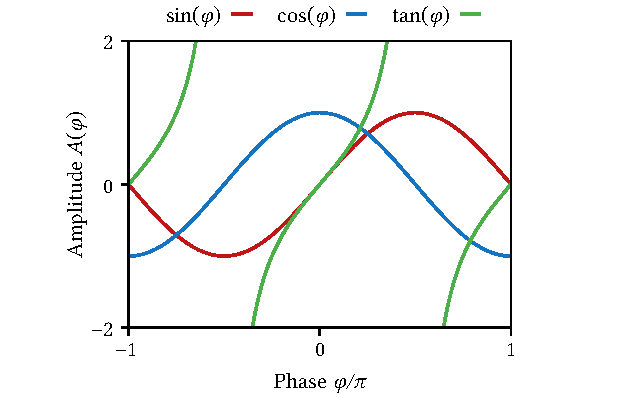
\includegraphics[width=0.2\textwidth]{test.jpg}
  \caption{This is simply a test figure, and some equation $\sin(2x)=1$, and some SI unit \SI{1.0e3}{m/s}, and some chemical \ce{CrO2}. This text can even be made even longer, since we want to test this properly.}
  \label{fig:test}
\end{figure}


Morbi non tortor volutpat, mattis odio at, tincidunt libero.
Donec pulvinar et mi at varius.
Sed vulputate lectus eu libero gravida, vel porta tortor bibendum.
Quisque dictum ex id quam ultrices, ut commodo nisl euismod.
Aliquam vulputate, urna quis sodales rhoncus, orci metus pulvinar velit, feugiat sollicitudin dui massa interdum tortor.
Nam sed ante vitae eros imperdiet bibendum.
Fusce pretium semper leo eget lobortis.
Sed dictum erat quis diam faucibus bibendum.
Integer vitae enim euismod, ornare augue quis, pharetra ante.
Phasellus venenatis tellus ut velit faucibus, posuere porttitor lacus hendrerit.

\begin{table}[h!]
  \centering
  \caption{This is simply a test table.}
  \label{tab:test}
  \begin{tabular*}{\dimexpr\textwidth-4em\relax}{@{\extracolsep{\stretch{1}}\,}lcc@{\,}}
    \toprule
    Name    &   Symbol    &   Value             \\
    \midrule
    Euler constant          & $e$   & $2.71...$  \\
    Circle constant         & $\pi$ & $3.14...$ \\
    Imaginary identity      & $i$ & $\sqrt{-1}$ \\
    \bottomrule
  \end{tabular*}
\end{table}

Lorem ipsum dolor sit amet, consectetur adipiscing elit.
Donec malesuada magna sem.
Fusce vitae lectus id magna convallis euismod.
Quisque viverra sollicitudin turpis, vel ultricies mauris dictum quis.
Praesent justo nunc, luctus in lectus in, placerat tempus orci.
Donec placerat neque ac tortor dignissim pellentesque.
Aenean tellus erat, eleifend id interdum a, volutpat et massa.
Quisque tristique accumsan efficitur.

Morbi non tortor volutpat, mattis odio at, tincidunt libero.
Donec pulvinar et mi at varius.
Sed vulputate lectus eu libero gravida, vel porta tortor bibendum.
Quisque dictum ex id quam ultrices, ut commodo nisl euismod.
Aliquam vulputate, urna quis sodales rhoncus, orci metus pulvinar velit, feugiat sollicitudin dui massa interdum tortor.
Nam sed ante vitae eros imperdiet bibendum.
Fusce pretium semper leo eget lobortis.
Sed dictum erat quis diam faucibus bibendum.
Integer vitae enim euismod, ornare augue quis, pharetra ante.
Phasellus venenatis tellus ut velit faucibus, posuere porttitor lacus hendrerit.

Lorem ipsum dolor sit amet, consectetur adipiscing elit.
Donec malesuada magna sem.
Fusce vitae lectus id magna convallis euismod.
Quisque viverra sollicitudin turpis, vel ultricies mauris dictum quis.
Praesent justo nunc, luctus in lectus in, placerat tempus orci.
Donec placerat neque ac tortor dignissim pellentesque.
Aenean tellus erat, eleifend id interdum a, volutpat et massa.
Quisque tristique accumsan efficitur.


\section{Continuation}
Morbi non tortor volutpat, mattis odio at, tincidunt libero.
Donec pulvinar et mi at varius.
Sed vulputate lectus eu libero gravida, vel porta tortor bibendum.
Quisque dictum ex id quam ultrices, ut commodo nisl euismod.
Aliquam vulputate, urna quis sodales rhoncus, orci metus pulvinar velit, feugiat sollicitudin dui massa interdum tortor.
Nam sed ante vitae eros imperdiet bibendum.
Fusce pretium semper leo eget lobortis.
Sed dictum erat quis diam faucibus bibendum.
Integer vitae enim euismod, ornare augue quis, pharetra ante.
Phasellus venenatis tellus ut velit faucibus, posuere porttitor lacus hendrerit.

Lorem ipsum dolor sit amet, consectetur adipiscing elit.\cite{feynman,statistics}\footnote{test}
Donec malesuada magna sem.
Fusce vitae lectus id magna convallis euismod.
Quisque viverra sollicitudin turpis, vel ultricies mauris dictum quis.
Praesent justo nunc, luctus in lectus in, placerat tempus orci.
Donec placerat neque ac tortor dignissim pellentesque.
Aenean tellus erat, eleifend id interdum a, volutpat et massa.
Quisque tristique accumsan efficitur.

Morbi non tortor volutpat, mattis odio at, tincidunt libero.
Donec pulvinar et mi at varius.
Sed vulputate lectus eu libero gravida, vel porta tortor bibendum.
Quisque dictum ex id quam ultrices, ut commodo nisl euismod.
Aliquam vulputate, urna quis sodales rhoncus, orci metus pulvinar velit, feugiat sollicitudin dui massa interdum tortor.\footnote{This is another footnote test.} %\footnote{This is simply just a simple test, with an equation $\sin \alpha = \cos(2a-1)/\cos(2a+1)$. And here is a chemical element \ce{CrO23} and physical unit \SI{12e3}{m}. }\footnote{Here is another footnote, also set in sans-serif.}%\footnote{$ABCDEFGHIJKLMOPQRSTUVWXYZ$ $abcdefghijklmopqrstuvwxyz$ $\alpha\beta\gamma\delta$ $\Gamma\Delta$ $\int_0^\infty \mathrm{d}x\,\sum_{ij} f(x_{ij}) \leq 0 \mathbf{xyz} \hat{x}+\check{y}\cdot\bar{u} \mathcal{F} \mathbf{x\sigma}$ \rmmath $\sin x$  $\cos x$}
Nam sed ante vitae eros imperdiet bibendum. 
Fusce pretium semper leo eget lobortis.
Sed dictum erat quis diam faucibus bibendum.
Integer vitae enim euismod, ornare augue quis, pharetra ante.
Phasellus venenatis tellus ut velit faucibus, posuere porttitor lacus hendrerit.

Lorem ipsum dolor sit amet, consectetur adipiscing elit.
Donec malesuada magna sem.
Fusce vitae lectus id magna convallis euismod.
Quisque viverra sollicitudin turpis, vel ultricies mauris dictum quis.
Praesent justo nunc, luctus in lectus in, placerat tempus orci.
Donec placerat neque ac tortor dignissim pellentesque.
Aenean tellus erat, eleifend id interdum a, volutpat et massa.
Quisque tristique accumsan efficitur.

Morbi non tortor volutpat, mattis odio at, tincidunt libero.
Donec pulvinar et mi at varius.
Sed vulputate lectus eu libero gravida, vel porta tortor bibendum.
Quisque dictum ex id quam ultrices, ut commodo nisl euismod.
Aliquam vulputate, urna quis sodales rhoncus, orci metus pulvinar velit, feugiat sollicitudin dui massa interdum tortor.
Nam sed ante vitae eros imperdiet bibendum.
Fusce pretium semper leo eget lobortis.
Sed dictum erat quis diam faucibus bibendum.\footnote{Test}
Integer vitae enim euismod, ornare augue quis, pharetra ante.
Phasellus venenatis tellus ut velit faucibus, posuere porttitor lacus hendrerit.


\chapter{Lorem ipsum}
\lipsum
\lipsum
\lipsum
\lipsum
\lipsum




\chapter{The Most Important Chapter}
\section{Here be random text about \textsc{srt/lrt}}
\lipsum




\backmatter
\printbibliography
\end{document}
